% Source : http://tex.stackexchange.com/questions/8879/draw-image-data-flow

\documentclass[]{article}
	\usepackage{tikz}
	\usetikzlibrary{positioning}


\begin{document}

%start tikzpicture,define a node style
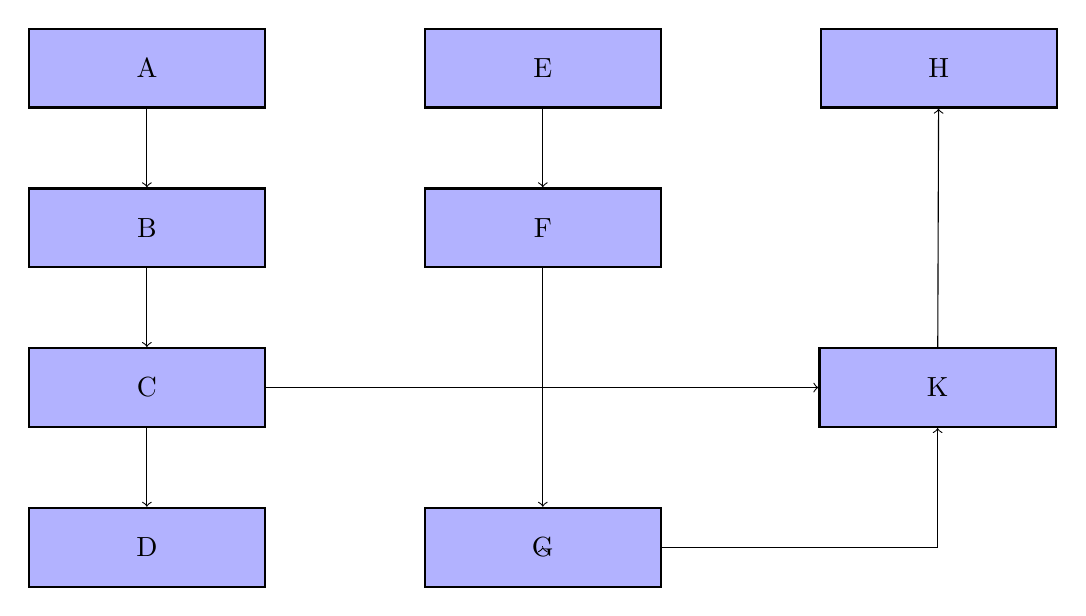
\begin{tikzpicture}[
	mystyle/.style={
		draw,rectangle,
		fill=blue!30,
		thick,
		minimum width=3cm,
		minimum height=1cm
	}
]
%start to define nodes relative to each other
	\node[mystyle] (A) {A};
	\node[mystyle] (B) [below=of A] {B};
	\node[mystyle] (C) [below=of B] {C};
	\node[mystyle] (D) [below=of C] {D};

%second column with a bit of a distance
	\node[mystyle,node distance=2cm] (E) [right=of A] {E};
	\node[mystyle,node distance=2cm] (F) [right=of B] {F};
	\node[mystyle,node distance=2cm] (G) [right=of D] {G};

	\node[mystyle,node distance=2cm] (H) [right=of E] {H};

%empty node for the gap in column 2 row 3
	\node[minimum width =3cm,node distance=2cm] (J) [right=of C] {};
	\node[mystyle,node distance=2cm] (K) [right=of J] {K};

%connect the nodes
	\draw[->] (A) -- (B);
	\draw[->] (B) -- (C);
	\draw[->] (C) -- (D);
	\draw[->] (G) -- (G);
	\draw[->] (E) -- (F);
	\draw[->] (F) -- (G);
	\draw[->] (G) -| (K);
	\draw[->] (K) -- (H);
	\draw[->] (C) -- (K);
\end{tikzpicture}

\end{document}
